\chapter{Sequences}
\section{What is a Sequence}
\subsection{Definition}
A sequence is a list of numbers in a specified order. The different numbers occurring in a sequence are called the terms of the sequence.\\
\[
    a_1,a_2,a_3,a_4\ldots,a_n
\]
Where the first term of the sequence is $a_1$, second term is $a_2$, n'th term is $a_n$.
We write a sequence using these notations:\\
\[
    a_n , \; (a_n), \; \{a_n\}, \; \{a_n\}_{n=1}^\infty
\]
Examples:\\
\begin{enumerate}
    \item $a_n = n = 1,2,3,4,\ldots$
    \item $a_n = n^2 = 1,4,9,16,\ldots$
    \item $a_n = (-1)^{n+1} = 1,-1,1,-1,\ldots$
    \item $a_n = \frac{1}{n} = 1,\frac{1}{2},\frac{1}{3},\frac{1}{4},\ldots$
    \item $a_n = \frac{(-1)^{n+1}}{n} = 1,-\frac{1}{2},\frac{1}{3},-\frac{1}{4},\ldots$
    \item $a_n = 1$ if $n$ is even, $n$ if $n$ is odd $= 1,1,3,1,5,1,7.\ldots$
    \item $a_n = 2,3,5,7,11,13,\ldots\;$ this is the sequence for prime numbers, it does not have a formula!
\end{enumerate}
\section{Limit Of A Sequence}
\subsection{Definition}
$L$ is the limit of a sequence $a_n$, or $a_n$ approaches $L\;$,$\lim_{n\to \infty} a_n = L,\: a_n\rightarrow L \iff$\\
$\forall\: \varepsilon>0 \:, \exists \: N\in \R,$ such that $\forall \: n>N \Longrightarrow |a_n - L|<\varepsilon$\\
Some people might be reading this and thinking what is all of this, so i'm gonna translate it for you.
For any positive number let's call it $\varepsilon$, there exists a number let's call it $N$ such that for any index that is bigger than that number $(N)$ the following happens $\Longrightarrow |a_n-L|<\varepsilon$, this is a literal translation from maths to english.\\\\

\subsection{Understanding The Limit}
Given any positive number $\varepsilon$, there exists a number $N$ such that for all indexes bigger than $N$ all the terms of the sequence apply this:\\
\[
    |a_n-L|<\varepsilon
\]
Which also means:
\[
    -\varepsilon<a_n-L<\varepsilon \quad \textbf{Feature 8}
\]
\[
    \iff
\]
\[
    L-\varepsilon<a_n<L+\varepsilon
\]
which means after a certain number $N$ all the terms of the sequence are going to be located between $L-\varepsilon$ and $L+\varepsilon$ or, $\forall \; \varepsilon>0 \; \exists \; N,$ such that $\forall\; n>N \Longrightarrow a_n\in (L-\varepsilon,L+\varepsilon)$

\subsection{Visually Seeing The Limit}
\noindent Examples:\\
If we look at the sequence $a_n = \frac{1}{n} = 1,\frac{1}{2},\frac{1}{3},\ldots$ we can tell that it approaches $0$, because the fractions are getting smaller and smaller each term.\\
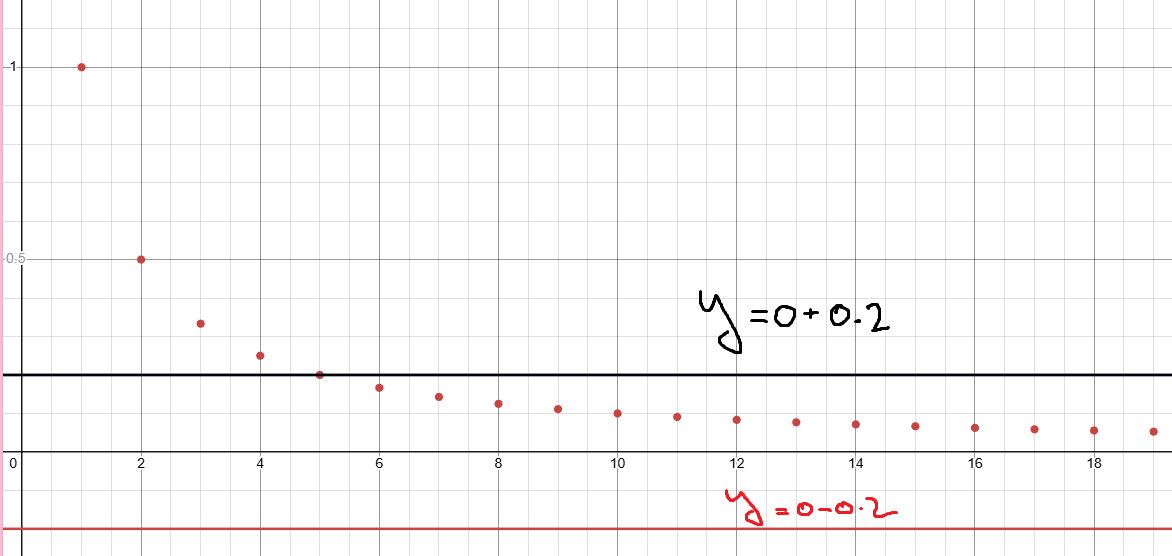
\includegraphics[scale = 0.7]{pictures/Graph1.png}
Given an $\varepsilon = 0.2$ $\exists\; N = 5,$ such that for all indexes bigger than $5\\ \Longrightarrow$ $0-0.2<a_n<0+0.2$\\
The definition of a limit states, that given any positive number $\varepsilon$, therefor we can pick any positive number $\varepsilon$ no matter how big and small it is, and there is always going to be a number $N$ such that for all the indexes bigger than $N$ such that $a_n\in(0-\varepsilon,0+\varepsilon)$\\\\
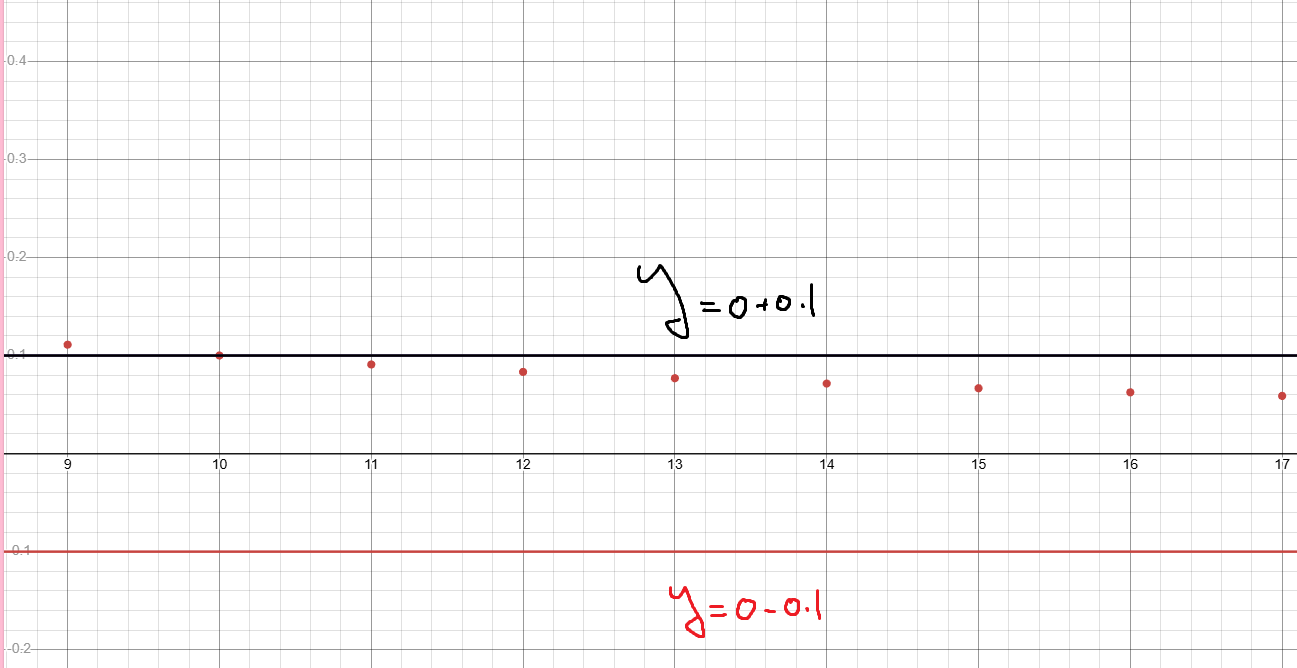
\includegraphics[scale=0.7]{pictures/Graph2.png}
Given an $\varepsilon = 0.1$ $\exists\; N = 10,$ such that for all indexes bigger than $10\\ \Longrightarrow$ $0-0.1<a_n<0+0.1$

\subsection{How To Prove The Limit Of A Sequence Is \(L\)}
To prove that \(\lim_{n \to \infty} a_n = L\), or that a sequence \(a_n\) approaches \(L\), we need to understand the definition of a limit.

\noindent In basic terms:  
For any positive number \(\varepsilon\), there exists a number \(N\) such that for all \(n > N\), the following holds:  
\[
|a_n - L| < \varepsilon.
\]

\noindent To prove that \(N\) exists, we need to find its value. Here's how I like to approach these types of proofs.

\subsubsection{Question 1: Proving \(\lim_{n \to \infty} \frac{1}{n} = 0\)}

Start by writing down the definition of a limit for this specific sequence:  
\[
\forall \; \varepsilon > 0, \; \exists \; N = \square \; \text{such that} \; \forall \; n > N \Longrightarrow
\]

We haven’t yet found \(N\), so we leave it blank for now. We want to prove that for all \(n > N\), the inequality holds:  
\[
|\frac{1}{n} - 0| = \frac{1}{n} < \varepsilon.
\]

Now, since \(n > N\), it follows that \(\frac{1}{n} < \frac{1}{N}\). So if we set \(\frac{1}{N} = \varepsilon\), this gives us:  
\[
\frac{1}{n} < \varepsilon \quad \text{and} \quad |\frac{1}{n} - 0| < \varepsilon.
\]

Finally, solving for \(N\) from \(\frac{1}{N} = \varepsilon\), we find:  
\[
N = \frac{1}{\varepsilon}.
\]

Thus, we can conclude the proof with the following:  
\[
\forall \; \varepsilon > 0, \; \exists \; N = \frac{1}{\varepsilon} \; \text{such that} \; \forall \; n > N \Longrightarrow |\frac{1}{n} - 0| < \varepsilon.
\]

\subsubsection{Question 2}
Another example: given a sequence $a_n = c ,\; c\in \R\;$ a constant sequence, we need to prove that $\lim_{n\to\infty}a_n = c$.\\
as we said we first write the definition while leaving $N$ blank to fill it in when we find it.\\
$\forall \; \varepsilon>0,\; \exists \; N = \square ,$ such that $\forall \; n>N \Longrightarrow$\\
\[
    |c-c| = 0 <\varepsilon
\]
for any input$(n)$, therefor $N$ can be any number, let's pick $1$
here's what the reader is gonna see after you fill in for $N=1$\\
$\forall \; \varepsilon>0,\; \exists \; N = 1 ,$ such that $\forall \; n>N \Longrightarrow$\\
\[
    |c-c|=0<\varepsilon
\]

\subsubsection{Question 3}
\noindent Another example: given the sequence $a_n = \frac{3n^2-5n+4}{n^2+4n-5},\;$ we need to prove that $\lim_{n\to\infty}a_n = 3$\\
Again, we start by writing the definition of a limit while leaving $N$ blank to fill it in when we find it.\\
$\forall\; \varepsilon>0\; \exists\;N = \square ,$ such that $\forall\; n>N\Longrightarrow$\\
\textbf{1st Step: Simplify The Expression}
\[
    |\frac{3n^2-5n+4}{n^2+4n-5}-3| = |\frac{3n^2-5n+4}{n^2+4n-5} -3\cdot\frac{n^2+4n-5}{n^2+4n-5}|=|\frac{3n^2-5n+4-3n^2-12n+15}{n^2+4n-5}|
\]
\[
    |\frac{-17n+19}{n^2+4n-5}| =|\frac{-1\cdot(17n-19)}{n^2+4n-5}| = |-1|\cdot|\frac{17n-19}{n^2+4n-5}| = |\frac{17n-19}{n^2+4n-5}| \quad \textbf{(Feature 5)}
\]
\textbf{2nd Step: Get Rid Of The Absolute Value}\\
We get rid of the Absolute Value by making whatever is inside the Absolute Value positive, \textbf{Reminder}: $|a| = a \iff a \geq 0$\\
If we look at a fraction $\frac{a}{b},\; b\neq 0$, if $a$ gets bigger, then the fractions it self gets bigger.\\
For all $n>2\Longrightarrow 17n-19>0 \Longrightarrow |17n-19|=17n-19<17n$
\[
    \Longrightarrow |\frac{17n-19}{n^2+4n-5}|=\frac{17n-19}{|n^2+4n-5|}<\frac{17n}{|n^2+4n-5|}
\]
For all $n>2$ the denominator $n^2+4n-5>0\Longrightarrow |n^2+4n-5| = n^2+4n-5$\\
$\forall\; n>2\Longrightarrow 4n-5>0 \iff n^2+4n-5>n^2\iff \frac{1}{n^2+4n-5}<\frac{1}{n^2}$ 
\[
    \frac{17n}{|n^2+4n-5|}<\frac{17n}{n^2}=\frac{17}{n}
\]
Where are looking for all the indexes $(n)>N \iff \frac{1}{n}<\frac{1}{N}$
\[
    \frac{17}{n}<\frac{17}{N}
\]
If $\frac{17}{N} = \varepsilon$ then the inital term $|\frac{3n^2-5n+4}{n^2+4n-5}-3|<\varepsilon \Longrightarrow \frac{17}{N}=\varepsilon \iff N=\frac{17}{\varepsilon}$
\[
    \frac{17}{n}<\frac{17}{N}<\varepsilon
\]
\textbf{3rd Step: Picking N}\\
All of this works if all the indexes are bigger than $2$, so we can't say that $N=\frac{17}{\varepsilon}$ is a valid answer, because we're saying that this statment works for every positive number $\varepsilon$, some values for $\frac{17}{\varepsilon}$ are less than $1$.\\
There is a solution for this.\\
$\forall\; \varepsilon>0 ,\; \exists\; N=max\{\frac{17}{\varepsilon},2\},$ such that $\forall\; n>N\Longrightarrow$
\[
    |\frac{3n^2-5n+4}{n^2+4n-5}-3|<\ldots<\frac{17}{N}<\varepsilon
\]
If $\frac{17}{\varepsilon}>2$ then if $N = \frac{17}{\varepsilon}\Longrightarrow |\frac{3n^2-5n+4}{n^2+4n-5}-3|<\varepsilon$\\
Otherwise, meaning if $\frac{17}{\varepsilon}\leq 2 \iff \frac{17}{2}\leq \varepsilon$ and for $N=2\Longrightarrow \frac{17}{N}=\frac{17}{2}\leq \varepsilon$\\